\chapter{Аналитическая часть}

\section{Модели описания объектов}


\section{Явление морфинга}
    Слово <<морфинг>> происходит от слова <<метаморфоза>>, которое, согласно 
    Согласно Оксфордскому словарю [All91], имеет следующее значение: "Процесс, в ходе которого кто-то/что-то полностью превращается во что-то другое".

    Таким образом, в случае трехмерных объектов термин <<морфинг>> можно интерпретировать как построение последовательности кадров, соответствующей постепенному переходу между двумя различными
    объектами, так называемыми исходными (начальными) и целевыми (конечными) моделями. На рисунке~\ref{fig:morhping_example} представлен пример морфинга трехмерных объектов.
    
    \begin{figure}[H]
		\centering
    	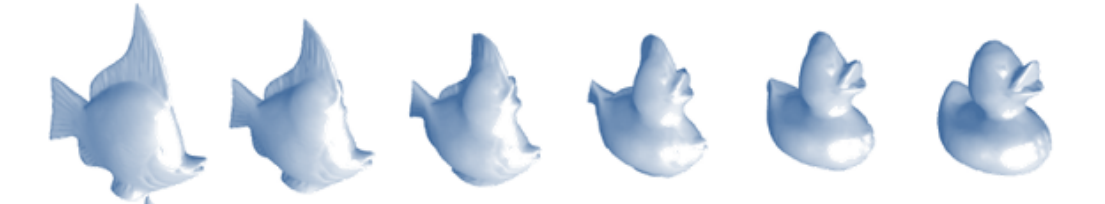
\includegraphics[width=\textwidth]{../inc/images/morhping_sequence}
    	\caption{TODO}
    	\label{fig:morhping_example}  
    \end{figure}

\section{Основные этапы морфинга}
	Поскольку фрукты в рамках данной работы представленны низколигональными трехмерными объектами без отверстий, что топологически эквивалентно сфере TODO: можно вообще такое писать без пояснения??, все по этапы будут рассмотрены для подобных объектов.
	
    % Процесс морфинга трехмерных объектов, представленных в виде полигональных сеток, можно разделить на три фундаментальных этапа, которые последовательно решают проблемы
    \begin{itemize}
    \item соответствия,
   	\item представления,
   	\item интерполяции.
    \end{itemize}
    
    \subsection{Установление соответствия между объектами}

    Ключевой и наиболее сложной задачей в процессе морфинга является установление соответствия между исходным и целевым объектами. Необходимо определить, как точки, ребра и грани одной модели соотносятся с элементами другой.
    
    \subsection{Параметризация на сферу}
    Чтобы сопоставить одну модель другой, необходимо выполнить их отображение в общее параметрическое пространство, а именно, единичную сферу. TODO: Как не закопаться?????
    
	\subsection{Параметризация звездообразных тел}
	\textit{Звездообразным} называется тело, которое имеет хотябы одну внутреннюю точку такую, что отрезки, соединяющие ее с вершинами тела, полностью лежат внутри фигуры \cite{alexa}.
	   
   Пусть точка $O$ видна из всех вершин тела $A$. Тогда, чтобы параметризовать тело $A$, необходимо перенесити его так, чтобы точка $O$ совпала с началом координат и нормировать координаты всех вершин.

	\subsection{Метод релаксации}
	Для параметризации произвольных объектов, топологически эквивалентных сфере, применяется итерационный метод релаксации \cite{alexa}. Метод основан на итеративном уточнении положений вершин.
	Процесс релаксации представлен на рисунке~\ref{fig:relaxation}. 
	
	В качестве исходного состояния создается грубая проекция модели на единичную сферу. Для этого вычисляется произвольная внутренняя точка объекта, которая принимается за центр сферы, после чего все вершины модели проецируются на ее поверхность. Начальная конфигурация, как правило, содержит значительные искажения и полигоны с некорректной ориентацией.
	
	На каждом раунде релаксации вершины сдвигаются к центру масс своих соседей:
	
	\begin{equation}
		v_i^{k + 1} = \frac{\sum_{j \in N(i)} v_j^{k}}{\parallel \sum_{j \in N(i)} v_j^{k} \parallel}, 
	\end{equation}
	
	где
	\begin{itemize}
		\item $v_i^{k + 1}$ --- новое положение $i$-ой вершины после $k$-го раунда релаксации;
		\item $v_i^{k}$ --- положение $i$-ой вершины на момент $k$-го раунда релаксации;
		\item $N(i)$ --- множество вершин, смежных с $i$-ой.
	\end{itemize}
	
	Для предотвращения коллапса всех вершин в одну точку после каждой итерации выполняется ре-центрирование всей сетки относительно начала координат:
	
	\begin{equation}
		v_i' = v_i - \frac{\sum_{j = 0}^{n} v_j}{n},
	\end{equation}
	
	где
	\begin{itemize}
		\item $v_i'$ --- новое положение $i$-ой вершины;
		\item $n$ --- количество вершин.
	\end{itemize}
	
	Релаксация прекращается, когда все полигоны на сфере приобретают ту же ориентацию, что и на исходной 3D-модели, что гарантирует отсутствие самопересечений и складок на поверхности.
	
	
	\begin{figure}[H]
		\centering
		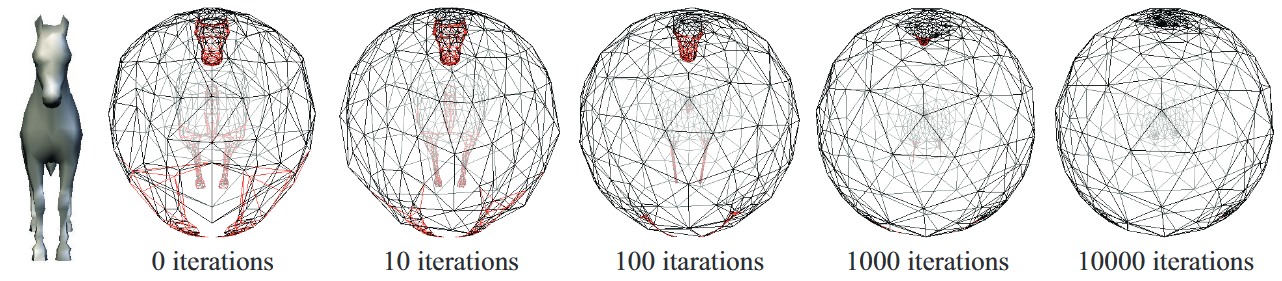
\includegraphics[width=\textwidth]{../inc/images/relaxation}
		\caption{Процесс релаксации сетки, красными отмечены грани c непрвильной ориентацией}
		\label{fig:relaxation}
	\end{figure}
	
	
    \subsection{Создание общего представления}
    После того как установлено соответствие, необходимо создать единую структуру, которая будет использоваться для всех промежуточных форм. Существует два основных подхода:
    \begin{itemize}
        \item \textit{Создание <<суперсетки>> (Map overlay)}\cite{alexa}: На параметрической сфере сетки накладываются друг на друга. В местах пересечения ребер создаются новые вершины, что формирует объединенную сетку, которая может принимать форму, как исходной так и целевой модели.
        \item \textit{Перестроение сетки (Remeshing)}\cite{alexa}: На основе прпметризации создается новая TODO
    \end{itemize}

    \subsection{Интерполяция геометрии}
    Заключительный этап --- вычисление траекторий движения вершин из их начального положения в конечное. Для каждой вершины общего представления необходимо вычислить ее координаты на исходной и целевой моделях. Процесс генерации промежуточных кадров сводится к интерполяции этих координат.

    Для определения начального и конечного положения каждой вершины общего представления используется метод, основанный на барицентрических координатах. Этот подход позволяет точно перенести положение точки из параметрического пространства на поверхность трехмерной модели.
    Процесс вычисления состоит из следующих шагов:
    \begin{itemize}
        \item поиск содержащего треугольника: Для каждой вершины общего представления определяется треугольник исходной (или целевой) сетки, в который она попадает в общем параметрическом пространстве (на сфере);
        \item расчет барицентрических координат: Вычисляются барицентрические координаты данной вершины относительно вершин найденного треугольника;
        \item проецирование в мировое пространство: полученные барицентрические координаты применяются к вершинам соответствующего треугольника, но уже на реальной модели.
    \end{itemize}

    После того как для всех вершин определены их начальные и конечные положения, для генерации промежуточных состояний морфинга применяется линейная интерполяция. Положение $P(t)$ каждой вершины в момент времени $t$, где t изменяется от 0 до 1, вычисляется по формуле:
    \begin{equation}
        P(t) = (1 - t) \cdot P_0 + t \cdot P_1,
    \end{equation}

    где
    \begin{itemize}
        \item $P_0$ --- начальное положение вершины,
        \item $P_1$ --- конечное положение вершины.
    \end{itemize}
    
    \section{Формализация объектов сцены}
    На сцене могут присутствовать следующие типы объектов:
    \begin{itemize}
    	\item источник света (задается положением в пространстве, цветом и интенсивностью света);
    	\item наблюдатель (задается положением в пространстве, точкой в пространстве, на которую направлен взгляд, направлением верха обзора TODO);
    	\item фрукт (задается моделью описания объектов, данными для этой модели, оптическими характеристиками поверхности);
    	\item результат морфинга (задается исходным и целевым объектами, стадией морфинга). 
    \end{itemize}
    
    Единовременно на сцене могут находиться либо один результат морфинга (сцена просмотра морфинга), либо два фрукта (сцена выбора исходного и целевого объекта). TODO?
    
    \section{Выбор модели описания объекта}
    
    
    
    \section{Анализ алгоритмов удаления невидимыъ линий и поверхностей}
    
    Алгоритмы удаления невидимых линий и поверхностей служат для удаления ребер, поверхностей или объемов, которые видимы или невидимы для наблюдателя, находящегося в заданной точке пространства\cite{rogers}.
    
    Самыми распространенными яляются: \textit{алгоритм Робертса}, \textit{алгоритм, использоующий z-buffer}, \textit{алгоритм трассировки лучей}.
    
   \subsubsection{Алгоритм Робертса}
   
   Данный алгоритм применим только к выпуклым телам. Если обрабатываемое тало невыпуклое --- его необходимо предварительно разбить на выпуклые.
   
   Алгоритм состоит из следующих этапов~\cite{rogers}:
   \begin{enumerate}
   	\item[1)] Удаление граней, экранируемых самим телом.
   	\item[2)] Удаление граней, экранируемых другими телами.
   	\item[3)] Удаление линий пересечения тел, экранируемых самими телами.
   \end{enumerate}
   
   \subsubsection{Алгоритм, использующий \textit{z-buffer}}
   
   Идея \textit{z}-буфера является обобщением идеи буфера кадра. Буфер кадра используется для запоминания аттрибутов (интенсивности) каждого пикселя в пространстве изображения. \textit{z}-буфер --- это отдельны буфер глубины, используемый для запоминания координаты \textit{z} каждого видимого пикселя в пространстве изображения\cite{rogers}.
   
   Этапы работы алгоритма~\cite{rogers}:
   
   \begin{enumerate}
   	\item[1)] Заполнить буфер кадра фоновым значением.
   	\item[2)] Заполнить z-буфер минимальным значением глубины.
   	\item[3)] Преобраз TODO: переход в куб камеры.
   	\item[4)] Для каждого пикселя ($x$, $y$), пренадлежащего телу вычислить его глубину $z(x, y)$.
   	\item[5)] Если глубина $z(x, y)$ > $z\textit{-буфер}(x, y)$, то записать атрибут текущего тела в $\textit{буфер-кадра}(x, y)$, записать глубину $z(x, y)$ в $z\textit{-буфер}(x, y)$.
   \end{enumerate}
   
   TODO: вывод по алгоритму
    
    \subsubsection{Алгоритм трассировки лучей}
    
    
    \section{Модель освещения}
    
    В компьютерной графике наиболее распространненными являются две модели освещения: \textit{локальную} и \textit{глобальную}~\cite{rogers}.
    
    Локальная модель учитывает только свет, падающий от источника (источников), и ориентацию поверхности~\cite{rogers}.
    
    Глобальная модель освещения учитывает также свет, отраженный от других объектов сцены или пропущенный через них~\cite{rogers}.
    
    Поскольку на сцене будет находиться только один объект, то будет использована локальная модель освещения.
    
    Интенсивность $I$ в точке $P$ в локальной модели вычисляется по формуле~\ref{eq:local_light_model}~\cite{rogers}.
    
    \begin{equation}
    	\label{eq:local_light_model}
    	I = k_aI_a + \frac{I_l}{d + K}[k_d(\mathbf{\hat{n}\cdot \hat{L}})+k_s(\mathbf{\hat{R}\cdot \hat{S}})^\alpha],
    \end{equation}
    
    где \\
    $k_a$ --- коэффициент \\
    $I_a$ --- интенсивность фонового освещения; \\
    $I_l$ --- интенсивность источника света; \\
    $d$ --- расстояние от источника света до точки~$P$; \\
    $K$ --- TODO; \\
    $k_d$ --- коэффициент диффузного отражения поверхности; \\
    $\mathbf{n}$ --- вектор нормали к поверхности в точке $P$; \\
    $\mathbf{L}$ --- вектор, обратный вектору падения луча; \\
    $k_s$ --- коэффициент зеркального отражения поверхности; \\
    $\mathbf{R}$ --- вектор, отраженного луча; \\
    $\mathbf{S}$ --- вектор, направленный на наблюдателя из точки $P$; \\
    $\alpha$ --- степень, аппроксимирующая пространственное распределение зеркально отраженного света.
        
    \section{Анализ алгоритмов закраски}
    
\section*{Вывод}

\clearpage